\documentclass[12pt]{article}
\setlength{\oddsidemargin}{0.25 in}
\setlength{\evensidemargin}{-0.25 in}
\setlength{\topmargin}{-0.6 in}
\setlength{\textwidth}{6.5 in}
\setlength{\textheight}{8.5 in}
\setlength{\headsep}{0.75 in}
\setlength{\parindent}{0 in}
\setlength{\parskip}{0.1 in}

%
% ADD PACKAGES here:
%

\usepackage{amsmath,amsfonts,amssymb,graphicx,mathtools}
\usepackage{multirow,url}

%
% The following commands set up the lecnum (lecture number)
% counter and make various numbering schemes work relative
% to the lecture number.
%
\newcounter{lecnum}
\renewcommand{\thepage}{\thelecnum-\arabic{page}}
\renewcommand{\thesection}{\thelecnum.\arabic{section}}
\renewcommand{\theequation}{\thelecnum.\arabic{equation}}
\renewcommand{\thefigure}{\thelecnum.\arabic{figure}}
\renewcommand{\thetable}{\thelecnum.\arabic{table}}

%
% The following macro is used to generate the header.
%
\newcommand{\lecture}[4]{
   \pagestyle{myheadings}
   \thispagestyle{plain}
   \newpage
   \setcounter{lecnum}{#1}
   \setcounter{page}{1}
   \noindent
   \begin{center}
   	\framebox{
   		\vbox{\vspace{2mm}
   			\hbox to 6.28in { {\bf MATH 254: Introduction to Statistics
   					\hfill #3} }
   			\vspace{4mm}
   			\hbox to 6.28in { {\Large \hfill Lesson #1: #2  \hfill} }
   			\vspace{2mm}
   			\hbox to 6.28in { {\hfill Corresponding Workbook Module: #4} }
   			\vspace{2mm}}
   	}
   \end{center}
   \markboth{Handout #1}{Handout #1}

   %{\bf Note}: {\it LaTeX template courtesy of UC Berkeley EECS dept.}

   %{\bf Disclaimer}: {\it These notes have not been subjected to the usual scrutiny reserved for formal publications.  They may be distributed outside this class only with the permission of the instructor.}
   %\vspace*{4mm}
   \vspace*{-4mm}
}
%
% Convention for citations is authors' initials followed by the year.
% For example, to cite a paper by Leighton and Maggs you would type
% \cite{LM89}, and to cite a paper by Strassen you would type \cite{S69}.
% (To avoid bibliography problems, for now we redefine the \cite command.)
% Also commands that create a suitable format for the reference list.
\renewcommand{\cite}[1]{[#1]}
\def\beginrefs{\begin{list}%
        {[\arabic{equation}]}{\usecounter{equation}
         \setlength{\leftmargin}{2.0truecm}\setlength{\labelsep}{0.4truecm}%
         \setlength{\labelwidth}{1.6truecm}}}
\def\endrefs{\end{list}}
\def\bibentry#1{\item[\hbox{[#1]}]}

%Use this command for a figure; it puts a figure in wherever you want it.
%usage: \fig{NUMBER}{SPACE-IN-INCHES}{CAPTION}
\newcommand{\fig}[3]{
			\vspace{#2}
			\begin{center}
			Figure \thelecnum.#1:~#3
			\end{center}
	}
% Use these for theorems, lemmas, proofs, etc.
\newtheorem{example}{Example}[lecnum]
\newtheorem{exercise}{Exercise}[lecnum]

\newtheorem{theorem}{Theorem}[lecnum]
\newtheorem{definition}[theorem]{Definition}
\newenvironment{proof}{{\bf Proof:}}{\hfill\rule{2mm}{2mm}}

% **** IF YOU WANT TO DEFINE ADDITIONAL MACROS FOR YOURSELF, PUT THEM HERE:

\newcommand\E{\mathbb{E}}

\begin{document}
%FILL IN THE RIGHT INFO.
%\lecture{**LECTURE-NUMBER**}{**DATE**}{**LECTURER**}{**SCRIBE**}
\lecture{6}{Simple Linear Regression with Inference for Slope}{Mintaek Lee}{6}
%\footnotetext{These notes are partially based on those of Nigel Mansell.}

% **** YOUR NOTES GO HERE:
\begin{example} (\textit{Testing whether the relationship between x and y is significant}) \\
	Suppose Mintaek wanted to know if the average number of hours students spend on social media per day is linearly related to their first year GPA or not. He randomly selects 30 students from a university and measures how many hours they spend on social media per day. Use the appropriate statistical methods and set up the hypotheses that best match Mintaek's interests.
\end{example}
	
We first need to recognize that \textbf{Social} (the average number of hours students spend on social media per day) is the explanatory/independent ($x$) variable and \textbf{GPA} (the first year GPA) is the response/dependent ($y$) variable. 

\noindent \textbf{Step 1}: Null and alternative hypotheses would then be:
\begin{itemize}
	\item $H_0$: $\beta_1 = 0$, the average number of hours students spend on social media per day and the first year GPA are NOT linearly related.
	\item $H_A$: $\beta_1 \neq 0$, the average number of hours students spend on social media per day and the first year GPA are linearly related.
\end{itemize}

\noindent \textbf{Step 2}: We now need to check conditions. For regression problems, we use the ``\textbf{LINE}''.

\begin{itemize}
	\item \textbf{L}inear: We need to make sure that the pattern looks linear. We can check this by observing the scatterplot.
	
	\begin{figure}[!h]
		\centering
		\vspace{-10 pt}
		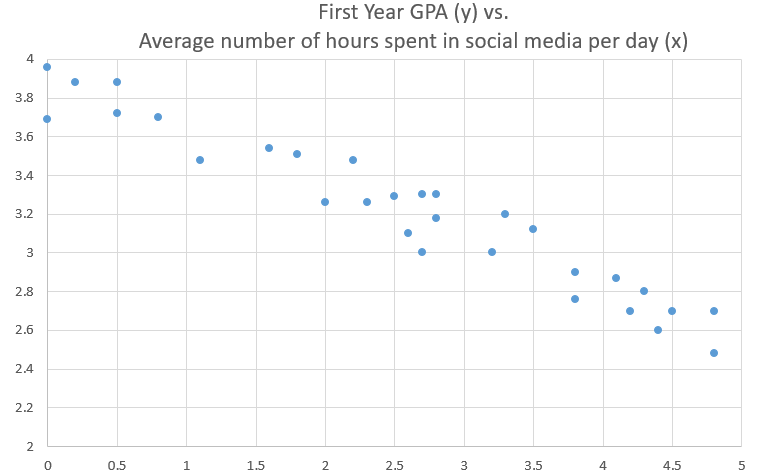
\includegraphics[width=10cm]{Figures/fig9.png}
		\vspace{-10 pt}
	\end{figure}

	Looking at the \textbf{scatterplot}, the relationship between $x$ and $y$ appear to be linear.
	
	\item \textbf{I}ndependent observations: We need to make sure that observations were collected independently (randomly). Since Mintaek selected 30 students randomly, we can say that this condition is met.
	
	\item \textbf{N}ormally distributed residuals: We need to make sure that residuals appear to have come from a normal distribution. We can check this by looking at the histogram of residuals.
	
	\begin{figure}[!h]
		\centering
		\vspace{-10 pt}
		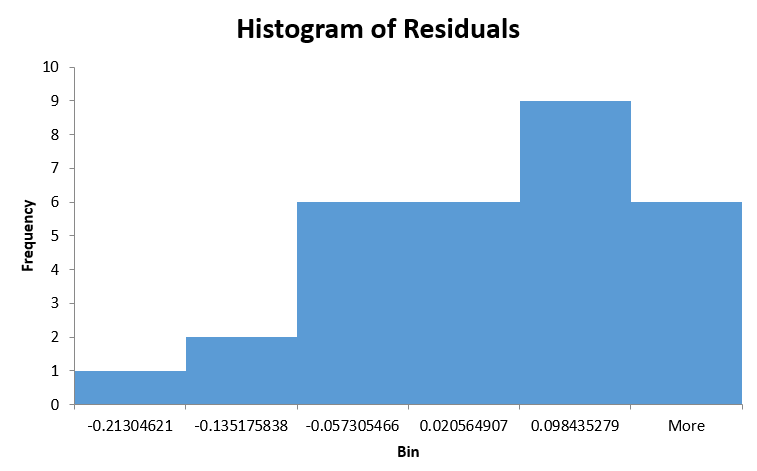
\includegraphics[width=10cm]{Figures/fig10.png}
		\vspace{-10 pt}
	\end{figure}
	
	Looking at the \textbf{histogram of residuals}, we see that the distribution of residuals appear to be fairly symmetric without any noticeable skewness. We can assume that this condition is met.
	
	\item \textbf{E}qual variation: We need to make sure that variation of residuals is consistent throughout the explanatory or independent ($x$) variables. We can check this by looking at the residual plot.
	
	\begin{figure}[!h]
		\centering
		\vspace{-10 pt}
		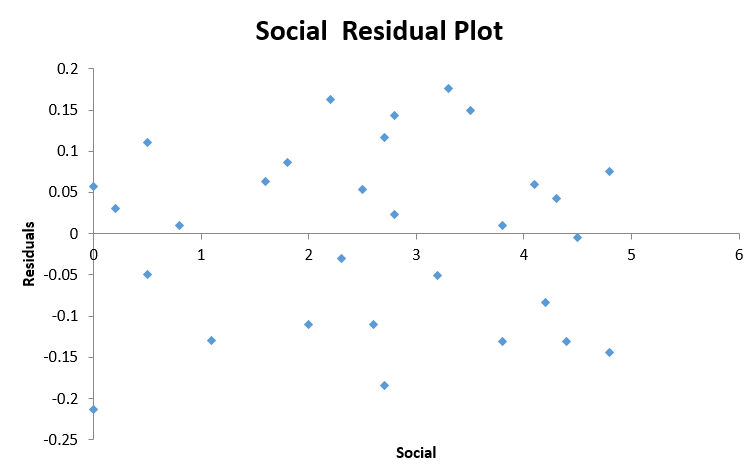
\includegraphics[width=10cm]{Figures/fig11.png}
		\vspace{-10 pt}
	\end{figure}
	
	Looking at the \textbf{residual plot}, we can see that variation of residuals is consistent throughout different $x$ values.
\end{itemize}

\vspace{10 pt}

\noindent \textbf{Step 3}: Since we verified all the necessary conditions, we can now fit the least squares regression line and find t-test statistic and P-value. You do not need to calculate any of them by hand. You will either be required to use software or appropriate outputs will be provided to you.

The software output for the regression analysis is shown below.

\begin{figure}[!h]
	\centering
	\vspace{-5 pt}
	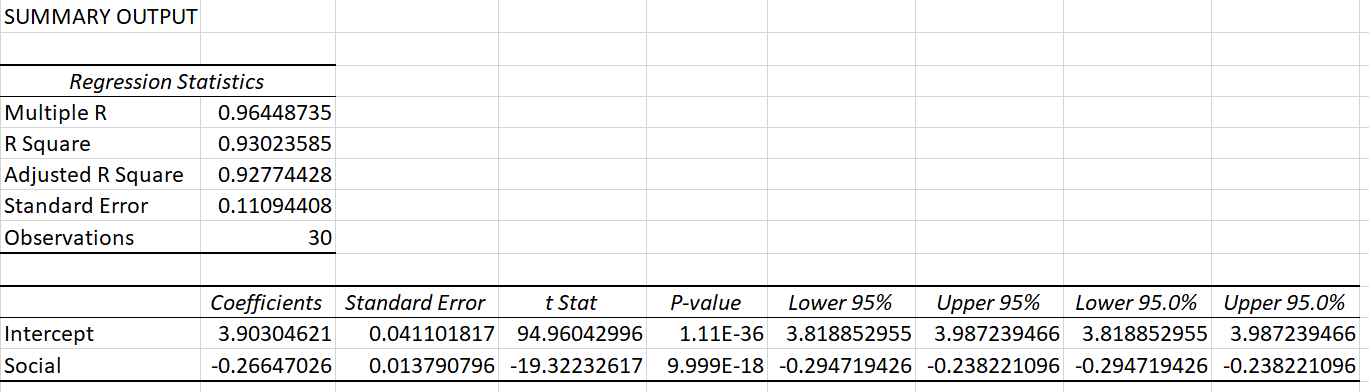
\includegraphics[width=\linewidth]{Figures/fig12.png}
	\vspace{-15 pt}
\end{figure}

From the output above, we find the t-test statistic value of $t = -19.3223$ and corresponding P-value of $9.999 \times 10^{-18}$ (approximately 0) for the slope term.

\vspace{10 pt}

\noindent \textbf{Step 4}: 

Since P-value was $9.999 \times 10^{-18}$ (approximately 0), thus smaller than the standard significance level $\alpha = 0.05$, we would reject our null hypothesis that the average number of hours students spend on social media per day and the first year GPA are NOT linearly related. Therefore, we conclude that there is significant evidence to suggest that the average number of hours students spend on social media per day and the first year GPA are linearly related.

\pagebreak

\begin{example}
	Since Mintaek verified that the average number of hours students spend on social media per day is linearly related to the first year GPA, he wants to make some inferences. Below are some short questions you can answer based on the findings above. Relevant software outputs are also shown below.

	\begin{figure}[!h]
		\centering
		\vspace{-10 pt}
		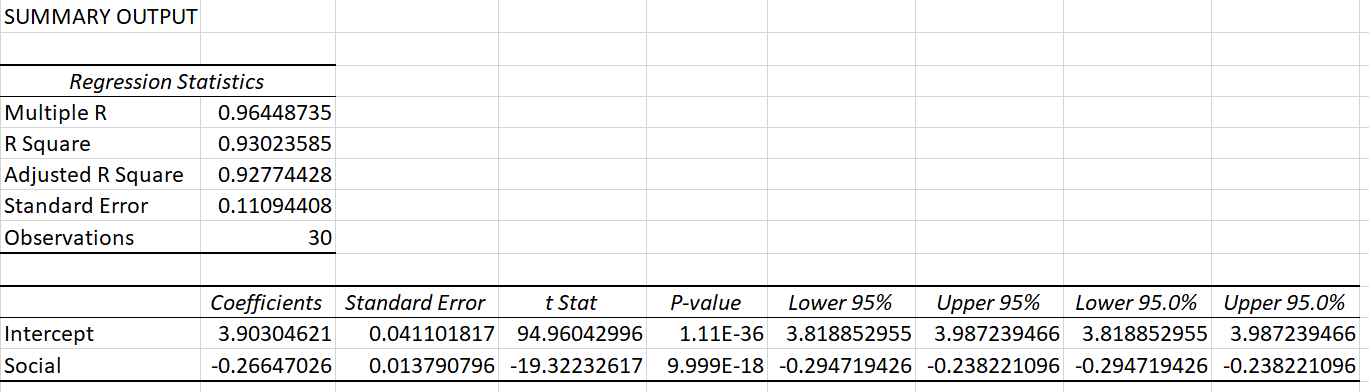
\includegraphics[width=\linewidth]{Figures/fig12.png}
		\vspace{-10 pt}
	\end{figure}
\end{example}

Technically, you still would need to check all conditions (LINE) for the simple linear regression. Since they were checked in Example 6.1, it will be omitted here.

\textit{\textbf{Part A.} Using the software output given above, find the least squares regression line for the given data.}

We look at the \textit{Coefficients} column on the bottom table. We see that the number corresponding to Intercept is 3.903, which is $b_0$ and the number corresponding to Parties is -0.266, which is $b_1$.

We therefore find $\hat{y} = b_1 +  b_0 \; x= 3.903 - 0.266 x$ as the least squares regression line for the given data.

\textit{\textbf{Part B.} Use the regression line for this data to predict the first year GPA of a student who spent 4 hours on social media per day on average.}

We substitute 4 into $x$ since $x$ was the explanatory variable (the average number of hours students spend on social media per day). We find $\hat{y} = 3.903 - 0.266 \times 4 = 2.84$.

A student who spent 4 hours on social media per day on average is predicted to have a first year GPA of 2.84.

\textit{\textbf{Part C.} Use the regression line for this data to predict the first year GPA of a student spend 15 hours on social media per day on average.}

This time, we find $\hat{y} = 3.903 - 0.266 \times 15 = -0.09$.

Note that 15 hours on social media per day is outside the given data range for average number of hours students who spent on social media per day. So, we don't necessarily know if the trend would continue to be linear for $x = 15$.  This is called an extrapolation which is a poor statistical practice. Furthermore, one cannot simply obtain a negative GPA. So we do not make a prediction for this student.

\end{document}

\begin{comment}
\begin{table}[!h]
\centering
\begin{tabular}{lll|lll|lll}
ID & Social & GPA & ID & Social & GPA & ID & Social & GPA \\ \hline
1  & 0     & 3.96  & 11 & 2.2   & 3.48  & 21 & 3.5   & 3.12  \\
2  & 0     & 3.69  & 12 & 2.3   & 3.26  & 22 & 3.8   & 2.90  \\
3  & 0.2   & 3.88  & 13 & 2.5   & 3.29  & 23 & 3.8   & 2.76  \\
4  & 0.5   & 3.88  & 14 & 2.6   & 3.10  & 24 & 4.1   & 2.87  \\
5  & 0.5   & 3.72  & 15 & 2.7   & 3.30  & 25 & 4.2   & 2.70  \\
6  & 0.8   & 3.70  & 16 & 2.7   & 3.00  & 26 & 4.3   & 2.80  \\
7  & 1.1   & 3.48  & 17 & 2.8   & 3.30  & 27 & 4.4   & 2.60  \\
8  & 1.6   & 3.54  & 18 & 2.8   & 3.18  & 28 & 4.5   & 2.70  \\
9  & 1.8   & 3.51  & 19 & 3.2   & 3.00  & 29 & 4.8   & 2.70  \\
10 & 2.0   & 3.26  & 20 & 3.3   & 3.20  & 30 & 4.8   & 2.48 
\end{tabular}
\end{table}
\end{comment}